\documentclass[10pt]{beamer}
%\documentclass[handout,10pt]{beamer} % printable version

\usepackage{../macros}


\title{Condtions et fonctions}

\hypersetup{
  pdftitle =  {Condtions et fonctions}
}

\begin{document}

\maketitle


%%%%%%%%%%%%%%%%%%%%%%%%%%%%%%%%%%%%%%%%%%%%%%%%%%%%%%%
\begin{frame}[fragile]
  \frametitle{Conditionnelle : la prise de décisions \texttt{if}}
  \alert{L'instruction conditionnelle if permet de prendre une décision.}

  \begin{block}{Dans l'éditeur}
    \begin{columns}[c]
      \begin{column}{0.53\textwidth}
  \begin{lstlisting}[style=editor]
a <- -2
if (a > 0) {
  paste(a,'est positif')
} else {
  paste(a,'est negatif ou nul')
}    
\end{lstlisting}

\end{column}
\begin{column}{0.47\textwidth}
  \RUN
  -2 est négatif ou nul
\end{column}
\end{columns} 
  \end{block}
  


\begin{block}{Au toplevel}
  C'est moins agréable, il faut faire attention au(x) saut(s) de ligne.
\end{block}
\begin{columns}[c]
\begin{column}{0.65\textwidth}
  \begin{lstlisting}
> a <- -2
> if(a>0) {paste(a,'est positif') }
> else {paste(a,'est negatif ou nul')}
  \end{lstlisting}
\end{column}
\begin{column}{0.35\textwidth}
  \RUN 
  \alert{Erreur : 'else' inattendu(e) in "else"}
\end{column}
\end{columns}
\end{frame}


\begin{frame}[fragile]
  \frametitle{Bloc et indentation}
  \begin{block}{Indentation}
    La bonne distance à la marge d'une ligne permet de structurer et de comprendre un programme.
        \newcommand{\indentrule}{\color{DarkBlue}\vrule\hspace{2pt}}        
  \begin{lstlisting}[style=editor, escapechar=?]
?\indentrule?a <- -2
?\indentrule?if (a > 0) {
?\indentrule?  ?\indentrule?paste(a,'est positif')
?\indentrule?} else {
?\indentrule?  ?\indentrule?paste(a,'est negatif ou nul')
?\indentrule?}    
\end{lstlisting}
 \end{block}

 \begin{block}{Bloc d'instructions}
   Un bloc d'instructions est une suite d'instructions alignées à la verticale.
   Il est nécessaire d’ouvrir et fermer les paires d’accolades : \{\dots\}.
   \begin{columns}[c]
     \begin{column}{0.58\textwidth}
       \newcommand{\indentrule}{\color{DarkBlue}\vrule\hspace{2pt}}        
       \begin{lstlisting}[style=editor, escapechar=?]
a <- -2
if (a > 0) {
  paste(a,'est positif')
else { 
  paste(a,'est negatif ou nul')
}    
\end{lstlisting}
\end{column}
\begin{column}{0.42\textwidth}
\RUN
\alert{Erreur : 'else' inattendu(e) in "else"}
\end{column}
\end{columns} 
\end{block}

\begin{center}
  \alert{Une utilisation correcte des accolades est obligatoire en R.}
\end{center}
\end{frame}

%%%%%%%%%%%%%%%%%%%%%%%%%%%%%%%%%%%%%%%%%%%%%%%%%%%%%%%
\begin{frame}[fragile]
  \frametitle{Opérateurs logiques : ET (\texttt{\&\&}) et OU (\texttt{||})}
  \begin{block}{Table de vérité : ces opérateurs ressemblent à ceux de la Logique.}
  \begin{table}
    \centering
    \begin{tabular}{|l|c|c|c|c|}
      \hline
      \texttt{p}        & \T & \T & \F & \F \\ \hline
      \texttt{q}        & \T & \F & \T & \F \\ \hline
      \texttt{p \&\& q} & \T & \F & \F & \F \\ \hline
      \texttt{p || q} & \T & \T & \T & \F \\ \hline
    \end{tabular}
  \end{table}
\end{block}


\begin{block}{Mais, ils sont court-circuités}
  \begin{lstlisting}[style=block]
> a <- -2
> x == 3
Erreur : objet 'x' introuvable
> (a > 0) && (x==3)
[1] FALSE    
\end{lstlisting}
L'expression \lstinline[columns=fixed]{x == 3} n'a pas été évaluée car \texttt{FALSE \&\& ? == FALSE}

La priorité de \texttt{\&\&} étant plus faible que celle des opérations arithmétiques,
on aurait pu écrire : \lstinline[columns=fixed]{a > 0 and x == 3} .

\end{block}
\end{frame}


%%%%%%%%%%%%%%%%%%%%%%%%%%%%%%%%%%%%%%%%%%%%%%%%%%%%%%%

\begin{frame}[fragile]
  \frametitle{Liens avec l'électronique numérique}
  \begin{block}{L'opérateur \texttt{||} est aussi court-circuité}
    
\begin{columns}[c]
\begin{column}{0.48\textwidth}
  \begin{lstlisting}[style=block]
> a <- -2
> x == 3
Erreur : objet 'x' introuvable
> (a < 0) || (x==3)
[1] TRUE    
\end{lstlisting}
\end{column}
\begin{column}{0.48\textwidth}
 car \texttt{TRUE || ? == TRUE}
\end{column}
\end{columns}
\end{block}

\begin{block}{Portes logiques en électronique} 
%\begin{figure}[h]
%  \centering
  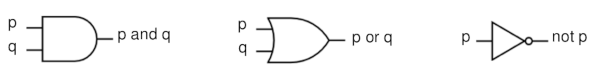
\includegraphics[width=0.8\textwidth]{portes-logiques} \\
%\end{figure}
L'opérateur \texttt{!} inverse les valeurs \texttt{TRUE} et \texttt{FALSE}. C'est l'inverseur \dots\\
Les constructeurs d'ordinateurs utilisent beaucoup la \alert{porte nand}.
  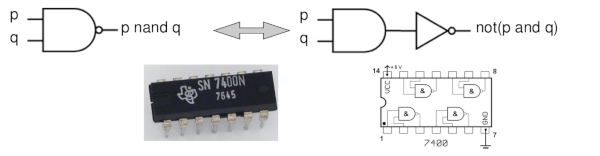
\includegraphics[width=0.8\textwidth]{porte-nand}  
\end{block}
\end{frame}


%%%%%%%%%%%%%%%%%%%%%%%%%%%%%%%%%%%%%%%%%%%%%%%%%%%%%%%
\begin{frame}[fragile]
  \frametitle{Les fonctions prédéfinies de R}
  Tous les langages de programmation fournissent un large ensemble de fonctions prêtes à être utilisées.
  \begin{exampleblock}{Exemples dans les entiers}
  \begin{lstlisting}[style=block]
> abs(-5) # la fonction "valeur absolue"
5
> '+'(4,9) # les opérateurs sont des fonctions cachées
13
\end{lstlisting}
\end{exampleblock}

Certaines fonctions résident dans des \alert{modules/packages} spécialisés, comme \texttt{TurtleGraphics} ou \texttt{shiny} \dots
\begin{lstlisting}
> turtle_forward(dist=15) # je veux réaliser un graphisme tortue
Erreur : impossible de trouver la fonction "turtle_forward"
> library(TurtleGraphics) # il faut charger l'extension
> turtle_init()
> turtle_forward(dist=15)  
\end{lstlisting}

\end{frame}  


%%%%%%%%%%%%%%%%%%%%%%%%%%%%%%%%%%%%%%%%%%%%%%%%%%%%%%%
\begin{frame}[fragile]
  \frametitle{Comment définir une nouvelle fonction ?}

  \begin{alertblock}{Syntaxte pour la définition d'une fonction}
  \begin{lstlisting}[style=edblock]
nomFonction <- function(listeDeParamètres) {
  blocInstructions
  return(résultatFonction)
}
\end{lstlisting}
Le mot \alert{return} signifie "le résultat est \dots".
\end{alertblock}

\begin{exampleblock}{Définir la fonction $f(n) \rightarrow 2n + 1$}
  \begin{lstlisting}[style=block]
> f <- function(n) {return( 2*n - 1)}
> f(5)
[1] 9    
\end{lstlisting}
\end{exampleblock}
\begin{block}{Paramètres non typés : \texttt{n} n'est pas forcément un entier.}
 \begin{lstlisting}[style=block]
> f(5.2) # avec des réels approchés
9.4
> f(complex(real = 1, imaginary = 1)) # avec des complexes
[1] 1+2i
  \end{lstlisting}  
\end{block}
\end{frame}


%%%%%%%%%%%%%%%%%%%%%%%%%%%%%%%%%%%%%%%%%%%%%%%%%%%%%%%
\begin{frame}[fragile]
  \frametitle{Les choix multiples avec \texttt{if \dots else if \dots else \dots}}
  
\begin{columns}[c]
\begin{column}{0.48\textwidth}
  \begin{lstlisting}[style=editor]
f <- function(x) {
  if( x < -1) return(-1)
  else if( x > 1) return(1)
  else return(x)
}   
\end{lstlisting}

ou de manière équivalente
\begin{lstlisting}[style=editor]
f <- function(x) {
  if( x < -1) return(-1)
  else {
    if( x > 1) return(1)
    else return(x)
}
\end{lstlisting}
\end{column}
\begin{column}{0.48\textwidth}
\begin{tikzpicture}
  % horizontal axis
  \draw[->] (-2,0) -- (2,0) node[anchor=north] {$x$};
  % vertical axis
  \draw[->] (0,-2) -- (0,2) node[anchor=east] {$y$};
  % labels
  \draw	(-1,0) node[anchor=south] {-1} (1,0) node[anchor=north] {1};
  \draw	(0,-1) node[anchor=west] {-1} (0,1) node[anchor=east] {1};
  % filter
  \draw[thick] (-2,-1) -- (-1,-1) -- (1,1) -- (2, 1);
  % dotted lines
  \draw[dotted] (-1,-1) -- (-1,0);
  \draw[dotted] (1,0) -- (1,1);
  
  \draw[dotted] (-1,-1) -- (0, -1);
  \draw[dotted] (0, 1) -- (1,1);
\end{tikzpicture}
\end{column}
\end{columns}




\end{frame}

\begin{frame}[fragile]
  \frametitle{Exemples}

  \begin{exampleblock}{Comment (re)définir la valeur absolue ?}
\begin{columns}[c]
\begin{column}{0.38\textwidth}
  \begin{lstlisting}[style=edblock]
Abs <- function(n) {
if(n>0) {
  return(n)
} else {
  return (-n)
}
\end{lstlisting}
\end{column}
\begin{column}{0.62\textwidth}
  \begin{lstlisting}
> paste('|-5| vaut', Abs(-5))
[1] "|-5| vaut 5"    
  \end{lstlisting}
\end{column}
\end{columns}
\end{exampleblock}

  \begin{exampleblock}{Comment (re)définir le maximum ?}
\begin{columns}[c]
\begin{column}{0.38\textwidth}
  \begin{lstlisting}[style=edblock]
Max <- function(n, m) {
if(n > m) {
  return(n)
} else {
  return (m)
}
\end{lstlisting}
\end{column}
\begin{column}{0.62\textwidth}
  \begin{lstlisting}
> paste('max(-10, -5) vaut', Max(-10, -5))
[1] "max(-10, -5) vaut 5"    
  \end{lstlisting}
\end{column}
\end{columns}
  \end{exampleblock}


\end{frame}


%%%%%%%%%%%%%%%%%%%%%%%%%%%%%%%%%%%%%%%%%%%%%%%%%%%%%%%
\begin{frame}
  \frametitle{Notions élémentaires sur les nombres premiers}
  \begin{block}{Nombre premier}
    Un nombre premier ne peut être divisé que par lui-même et par 1.
  \end{block}
  \begin{block}{Plus grand commun diviseur (PGCD)}
    Le PGCD de deux nombres entiers non nuls est le plus grand entier qui les divise simultanément. 
  \end{block}

  \begin{block}{Premiers entre eux}
    on dit que deux entiers sont premiers entre eux si leur plus grand commun diviseur est égal à 1.
  \end{block}

  Supposons que la fonction \texttt{gcd(p, q)} existe et renvoie le plus grand diviseur commun des entiers \texttt{p} et \texttt{q} (nous la programmerons en TP).
\end{frame}

%%%%%%%%%%%%%%%%%%%%%%%%%%%%%%%%%%%%%%%%%%%%%%%%%%%%%%%
\begin{frame}[fragile]
  \frametitle{Composition de fonctions I}
  Créons une fonction \texttt{premiersEntreEux(p,q)} basée sur la fonction \texttt{gcd}.
  \begin{lstlisting}[style=editor]
premiersEntreEux <- function(p,q) {
  if (gcd(p,q) == 1) {
    return(TRUE)
  } else {
    return(FALSE)
  }
}    
\end{lstlisting}
ou encore
\begin{lstlisting}[style=editor]
premiersEntreEux <- function (p,q) {
  if (gcd(p,q) == 1) {
    return(TRUE)
  }
  return(FALSE)
}  
\end{lstlisting}
Le mot clé \alert{\texttt{return} provoque un échappement}. 
Le reste du texte de la fonction est abandonné !

\end{frame}


%%%%%%%%%%%%%%%%%%%%%%%%%%%%%%%%%%%%%%%%%%%%%%%%%%%%%%%
\begin{frame}[fragile]
  \frametitle{Composition de fonctions II}
 
Une version qui renvoie directement le résultat de l'évaluation de l'expression.
\begin{lstlisting}[style=editor]
premiersEntreEux <- function(p,q) {
  return(gcd(p,q) == 1)
}  
\end{lstlisting}

Une version encore plus courte qui omet les accolades et \texttt{return}.
\begin{lstlisting}[style=editor]
premiersEntreEux <- function(p,q) gcd(p,q) == 1
\end{lstlisting}

\begin{lstlisting}
> premiersEntreEux(21,6)
[1] FALSE
> premiersEntreEux(21,8)
[1] TRUE  
\end{lstlisting}

Vous voyez qu'il existe différentes manières de coder une fonction.
Elles se distinguent par leur \alert{efficacité}, mais aussi leur \alert{élégance}.


\end{frame}


%%%%%%%%%%%%%%%%%%%%%%%%%%%%%%%%%%%%%%%%%%%%%%%%%%%%%%%
\begin{frame}[fragile]
  \frametitle{Documenter une fonction}
  \begin{block}{Pour l'instant}
    Ajouter simplement des commentaires au début de la fonction.    
  \end{block}

\begin{lstlisting}
premiersEntreEux <- function(p,q) {
  # Détermine si deux entiers p et q sont premiers entre eux par calcul du PGCD.
  #
  # Arguments:
  #  p un entier
  #  q un entier
  #
  # Returns: TRUE si p et q sont premiers entre eux, et FALSE sinon.
  ...
}
\end{lstlisting}
En effet, il suffit de \alert{taper le nom d’une fonction pour voir son code}.
\end{frame}

%%%%%%%%%%%%%%%%%%%%%%%%%%%%%%%%%%%%%%%%%%%%%%%%%%%%%%%
\begin{frame}[fragile]
  \frametitle{Consulter la documentation de R}

  \begin{lstlisting}
> ?paste # consulter la documentation d'une fonction
Concatenate Strings

Description:

     Concatenate vectors after converting to character.

Usage:

     paste (..., sep = " ", collapse = NULL)
     paste0(..., collapse = NULL)
     
Arguments:
 ...    
> ??paste # rechercher dans la documentation
  \end{lstlisting}
\end{frame}  


% \begin{frame}[fragile]
%   \frametitle{Test Code R}
%   \begin{lstlisting}[caption={My Caption}]
%     print(sample(1:3))
%     print(sample(1:3, size=3, replace=FALSE))  # same as previous line
%     print(sample(c(2,5,3), size=4, replace=TRUE)
%     print(sample(1:2, size=10, prob=c(1,3), replace=TRUE))    
%   \end{lstlisting}


%   \begin{exampleblock}{Code dans block}
%       \begin{lstlisting}
% print(sample(1:3))
%     print(sample(1:3, size=3, replace=FALSE))  # same as previous line
%     print(sample(c(2,5,3), size=4, replace=TRUE)
%     print(sample(1:2, size=10, prob=c(1,3), replace=TRUE))
%     x <- 5
%     if(x > 0){
%       print("Positive number")
%     }
%   \end{lstlisting}
%   \end{exampleblock}
% \end{frame}


%%%%%%%%%%%%%%%%%%%%%%%%%%%%%%%%%%%%%%%%%%%%%%%%%%%%%%%
 \questionSlide

%%%%%%%%%%%%%%%%%%%%%%%%%%%%%%%%%%%%%%%%%%%%%%%%%%%%%%%
 \appendix
 \backupSlides
%%%%%%%%%%%%%%%%%%%%%%%%%%%%%%%%%%%%%%%%%%%%%%%%%%%%%%%

%%%%%%%%%%%%%%%%%%%%%%%%%%%%%%%%%%%%%%%%%%%%%%%%%%%%%%%
% \begin{frame}[fragile]{Backup slides}
%   Sometimes, it is useful to add slides at the end of your presentation to
%   refer to during audience questions.

%   The best way to do this is to include the \verb|appendixnumberbeamer|
%   package in your preamble and call \verb|\appendix| before your backup slides.

%   will automatically turn off slide numbering and progress bars for
%   slides in the appendix.
% \end{frame}


%%%%%%%%%%%%%%%%%%%%%%%%%%%%%%%%%%%%%%%%%%%%%%%%%%%%%%%
% \begin{frame}[allowframebreaks]{References}

%   % \bibliography{../bib_parallelism,../bib_others}
%   % \bibliographystyle{abbrv}

% \end{frame}

\end{document}

%%% Local Variables:
%%% mode: latex
%%% TeX-master: t
%%% End:
